\documentclass[letterpaper]{article}
\usepackage[spanish]{babel}
\usepackage[utf8]{inputenc}
\usepackage{graphicx}
\usepackage{amsmath}

\title{Proyecto de Ingeniería de Software II}
\author{Acuña Yeomans Eduardo\\Contreras Mejía Daniel\\Valle Ruiz Francisco Manuel}
\date{Lunes 2 de Junio del 2014}

\begin{document}

\maketitle

%%%
\section{Presentación}

\subsection{Sobre Sabrosoftware}
Sabrosoftware es la compañía ficticia de desarrollo de software con mayor prestigio en la clase de Ingeniería de Software II impartida por el profesor Adrián en la segunda mitad del año 2014. Engendrada en el 2013 como parte de un proyecto de Ingeniería de Software I, Sabrosoftware ha aprendido de sus errores en el previo trabajo y planea posicionarse como la compañía ficticia de desarrollo de software de toda la región sur-este de la Universidad de Sonora campus Hermosillo.

\begin{figure}[h!]
  \centering
    
\includegraphics[width=0.7\textwidth]{LogoSabrosoftware}
    \caption{Logo de Sabrosoftware}
\end{figure}

\subsection{Sobre el equipo}
El equipo de trabajo es conformado por tres estudiantes de la licenciatura en Ciencias de la Computación:

\subsubsection*{Eduardo Acuña Yeomans}
Estudiante de sexto semestre, he escrito pequeños programas y trabajando con los otros integrantes de Sabrosoftware dentro y fuera del ámbito escolar.

Tiene experiencia moderada en los lenguajes de programación de C, C++ y Scheme.
Tiene poca experiencia en los lenguajes de programación de Java y Python.

\subsubsection*{Daniel Contreras Mejía}
Estudiante del octavo semestre, entusiasta en el área de la computación nivel amateur; cuenta con experiencia media en Ruby, C++, C\#, HTML, CSS y es fluido en el lenguaje Inglés a nivel profesional.

\subsubsection*{Francisco Manuel Valle Ruiz}
Estudiante del sexto semestre, se graduó del bachillerato con especialidad técnica en Informática (2008 - 2011) y experiencia media en C++, HTML, CSS 

\subsection{Flujo y relaciones de trabajo}
\begin{itemize}
\item \textbf{Líder del proyecto:} Eduardo Acuña Yeomans
\item \textbf{Encargado del diseño interfaz:} Daniel Contreras Mejía
\item \textbf{Encargado del diseño algorítmico:} Francisco Manuel Valle Ruiz
\item \textbf{Encargado de documentación:} Eduardo Acuña Yeomans
\item \textbf{Encargado de pruebas:} Francisco Manuel Valle Ruiz
\item \textbf{Encargado de mantenimiento técnico:} Daniel Contreras Mejía 
\end{itemize}

El flujo de comunicación y trabajo se basa en desarrollo de documentos y códigos en plataformas colaborativas como Google Docs y GitHub, así como el uso de una lista de correos.

%%%
\section{Descripción del Proyecto}
El problema planteado por el profesor Adrián es el de envío y recepción de oficios por parte de profesores y administrativos de la Universidad de Sonora. Nos mostró que la mayoría de los oficios que se redactan tienen practicamente el mismo formato y que el procedimiento de recepción es el de mandar el oficio al destinatario y que al llegar a la oficina correspondiente el oficio sea sellado de \emph{recibido}.

Se plantea desarrollar un sistema que emule este procedimiento. Las ideas que se mencionaron en clase fueron de generar documentos en formato PDF y manejar una especie de bandeja virtual para clasificar los documentos como recibidos o no recibidos, así como simplificar el proceso de darle formato a los oficios; se entendió que esta parte del sistema funcionara como el ``visto'' del facebook.

%%%
\section{Presupuestación}
La presupuestación del proyecto se realizó de dos maneras:

\subsection{En base a Líneas de Código}
Separamos el proyecto en diferentes secciones para poder aproximarnos a una mejor aproximación:

\begin{itemize}
\item Interfaz gráfica \textbf{LDC: 500}
\item Procesamiento de entradas \textbf{LDC: 100}
\item Generación de documentos \textbf{LDC: 500}
\item Procesamiento de salidas \textbf{LDC: 100}
\item Intercambio de documentos entre usuarios \textbf{LDC: 200}
\end{itemize}

Esta asignación numérica resulta con un total de \textbf{1400} líneas de código. Asumiendo que el sueldo mensual por persona es de $\$5,000^{00}$ y que la cantidad de líneas de código al mes son 90. Determinamos que el precio por línea de código es de $\$55^{00}$. Por lo tanto, el presupuesto estimado del proyecto, basandonos en líneas de código es de $\$77,000^{00}$.

\subsection{En base a Puntos de Función}
Al obtener los \emph{puntos de función} totales del proyecto se establecerán una serie de medidas para poder realizar la estimación del presupuesto.

\begin{enumerate}
\item \textbf{Entradas externas}
  \begin{itemize}
  \item Datos del oficio a mandar
  \item Datos del usuario
  \end{itemize}
\item \textbf{Salidas externas}
  \begin{itemize}
  \item Interfaz gráfica
  \item Mensajes de error
  \item Visualización de documentos
  \end{itemize}
\item \textbf{Consultas externas}
\item \textbf{Archivos lógicos internos}
  \begin{itemize}
    \item Estructura del formato
    \item Estructura del contenido del oficio
    \item Red de contactos por usuario
  \end{itemize}
\item \textbf{Archivos de interfaz externas}
  \begin{itemize}
  \item Datos de los usuarios
  \end{itemize}
\end{enumerate}

Ya que no se ha realizado un proyecto como este, se estimaron como tareas ``promedio'' y es así como se ponderan estos dominios para el conteo de los puntos de función. Por lo que el \emph{conteo total ponderado} resulta 60.

Se establecen los factores de ajuste:

\begin{enumerate}
\item ¿El sistema requiere respaldo y recuperación confiable? \textbf{2}
\item ¿Comunicación de datos especializada es requerida para la transferencia de información? \textbf{0}
\item ¿Hay funciones de procesamiento distribuido? \textbf{0}
\item ¿Es el rendimiento crítico? \textbf{1}
\item ¿El sistema será ejecutado en ambientes altamente utilizados? \textbf{2}
\item ¿Requiere entradas de datos en línea? \textbf{5}
\item ¿Se requieren múltiples pantallas u operaciones para la transacción de información en línea? \textbf{1}
\item ¿Los archivos lógicos internos son actualizados en línea? \textbf{3}
\item ¿Hace uso de archivos de entrada/salida complejos? \textbf{2}
\item ¿Realiza procesamiento interno complejo? \textbf{2}
\item ¿El código está diseñado para ser reutilizado? \textbf{2}
\item ¿Se incluye instalación y conversión en el diseño? \textbf{0}
\item ¿El sistema está diseñado para múltiples instalaciones en diferentes organizaciones? \textbf{0}
\item ¿La aplicación está diseñada para facilitar cambios y fácil uso por el usuario? \textbf{0}
\end{enumerate}

Dada esta valoración el \emph{total de factores de ajuste} es \textbf{20}; para obtener el valor de \emph{puntos de función (PF)} se usa la fórmula:
\begin{align*}
  PF &= ConteoPonderado \times [0.65+0.01 \times ConteoAjuste] \\
  PF &= 60 \times [0.65 + 0.01 \times 20] \\
  PF &= 60 \times [0.65 + 0.2] \\
  PF &= 60 \times 0.85 \\
  PF &= 51
\end{align*}

En teoría este valor numérico es útil conociendo información sobre los integrantes del equipo de trabajo como:
\begin{itemize}
\item Promedio de líneas de código por PF.
\item Promedio de PF al mes.
\item Promedio de errores por PF.
\end{itemize}

Sin embargo, estos datos no se tienen en un primer proyecto, por lo tanto esta estimación será ajustada conforme se avance el proyecto y conforme se desarrollen mas proyectos. Estos primeros valores son relacionados con la estimación de líneas de código, la cual también está basada en una idea muy vaga del proyecto:

\begin{itemize}
\item Promedio de líneas de código por PF: \textbf{27.45}
\item Promedio de PF al mes: \textbf{3.28}
\end{itemize}

%%%
\section{Ámbito y Descomposición del software}
\subsection{Ámbito del proyecto}
Actualmente en la Universidad de Sonora, varios procedimientos oficiales requieren el envío de oficios. Usualmente estos oficios son documentos con un formato determinado que un empleado redacta para imprimirlo y mandarlo a algún otro empleado u oficina de la Universidad, cuando este documento es recibido por el destinatario es sellado de recibido para tener como constancia que la comunicación se efectuó de manera oficial.

Dado que hay varias partes de este proceso que se pueden automatizar, se plantea elaborar un sistema que pueda emular esta comunicación oficial de manera virtual, comprendiendo la redacción del oficio, la entrega al destinatario y el sellado de recibido.

\subsection{Descomposición del proyecto}
El proyecto se compone fundamentalmente en tres partes:
\begin{itemize}
\item \textbf{Captura de información:} Emisor, receptor y contenido del oficio.
\item \textbf{Procesamiento de información:} Transformar la estructura básica en un oficio con el formato usual.
\item \textbf{Envío y sellado:} Entrega virtual del documento al destinatario y confirmación de recibido cuando el destinatario consulte los oficios pendientes.
\end{itemize}

La \emph{captura de información} se encarga de determinar que los datos ingresados sean válidos, se contempla la implementación de una interfaz de usuario gráfica en una página web.

El \emph{procesamiento de información} consistirá de varios algoritmos que manejarán una estructura determinada de los datos para realizar un acomódo adecuado con el formato del oficio establecido. El resultado de este proceso es un archivo en formato PDF.

El \emph{envío y sellado} se encargará de informar a otro usuario que un documento en PDF le fué enviado y al momento de que este usuario revise el PDF se actualizará el documento como recibido.

Se opta por desarrollar una aplicación web para la implementación de este sistema. La ventaja es tanto para el usuario como para los desarrolladores ya que no será necesario descargar un programa para utilizar el sistema y los desarrolladores tendrán un control sobre toda la información debido a que será alojada en un servidor web.

%%%
\section{Planificación}

\subsection{Análisis y selección de modelo}
Se utiliza el modelo por \emph{prototipos} ya que el cliente solo planteó una idea general del programa y será útil para los desarrolladores ir dejando los detalles sutiles para el final (debido a la poca experiencia que se tiene con este tipo de proyectos).

\subsection{Lista de actividades}

\begin{enumerate}
\item[1] \textbf{Analizar el problema: (3 días)}
  \begin{enumerate}
  \item[1.1] Reunión con el cliente.
  \item[1.2] Aplicar un cuestionario de espectativas.
  \item[1.3] Determinar los puntos clave del sistema.
  \end{enumerate}
\item[2] \textbf{Diseñar el primer prototipo: (3 semanas)}
  \begin{enumerate}
  \item[2.1] Determinar el cuerpo de conocimiento requerido y establecer las técnicas o métodos que el equipo debe aprender.
  \item[2.2] Establecer la interacción entre los diferentes componentes del software.
  \item[2.3] Analizar la manera en como el usuario interaccionará con el sistema.
  \item[2.4] Diseñar la interfaz de usuario.
  \item[2.5] Elegir o diseñar los algoritmos de generación de formato.
  \item[2.6] Elegir o diseñar los algoritmos de generación de archivos PDF.
  \item[2.7] Implementar el sistema.
  \end{enumerate}
  
  \item[3] \textbf{Pruebas al prototipo: (1 semana)}
    \begin{enumerate}
    \item[3.1] Probar el software con usuarios ficticios.
    \item[3.2] Probar el software con entradas usuales.
    \item[3.3] Probar el software con entradas erráticas.
    \end{enumerate}
    
  \item[4] \textbf{Correcciones: (1 semana)}
    \begin{enumerate}
    \item[4.1] Corregir validación de datos.
    \item[4.2] Corregir algoritmos de transformación.
    \item[4.3] Corregir interfaz de usuario.
    \end{enumerate}
    
  \item[5] \textbf{Documentación: (4 semanas)}
    \begin{enumerate}
    \item[5.1] Documentación de usuario.
    \item[5.2] Documentación de desarrolladores.
    \item[5.3] Informe para el cliente.
    \end{enumerate}

  \item[6] \textbf{Reunión con el cliente: (2 días)}
    \begin{enumerate}
    \item[6.1] Presentación del prototipo.
    \item[6.2] Anotación de cambios o mejoras.
    \end{enumerate}
  \item[] \textbf{...}
\end{enumerate}

\subsection{Red de tareas}
En la \emph{Figura 2} se aprecia la dependencia de las actividades.
\begin{figure}[h!]
  \centering
  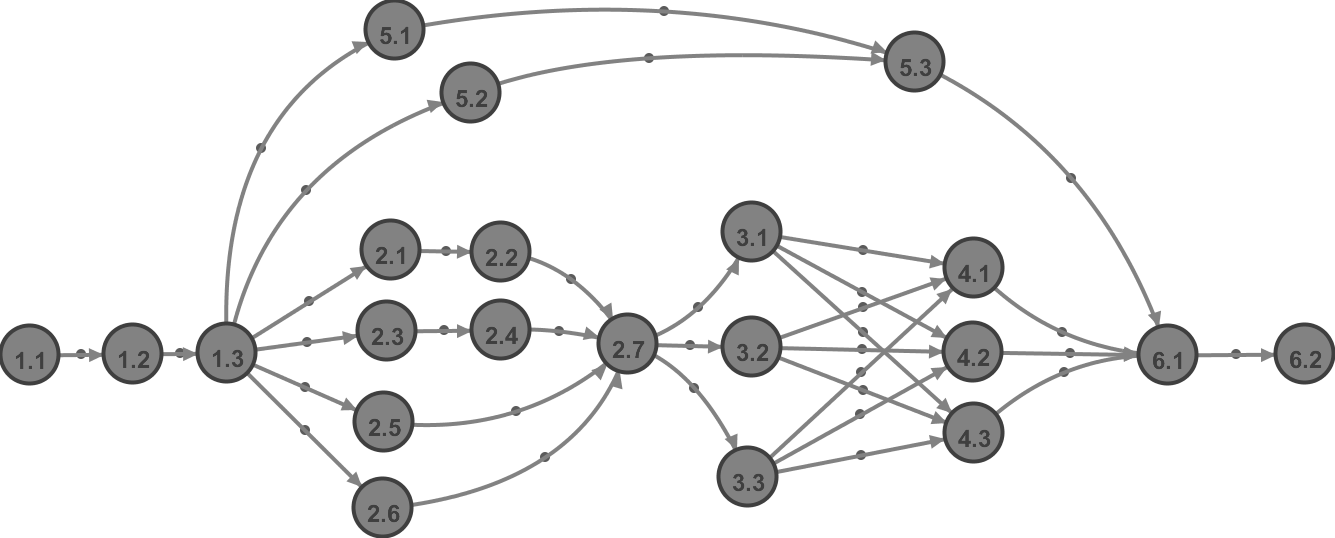
\includegraphics[width=1\textwidth]{RedTareas}
  \caption{Dependencia de tareas}
\end{figure}

\subsection{Carga de trabajo}
\begin{itemize}
\item \textbf{Acuña Yeomans Eduardo:} 1.1, 1.2, 1.3, 2.7, 5.1, 5.2, 5.3, 6.1, 6.2.
\item \textbf{Contreras Mejía Daniel:} 1.1, 2.1, 2.2, 2.3, 2.4, 2.7, 4.1, 4.3, 6.1.
\item \textbf{Valle Ruiz Francisco Manuel:} 1.1, 2.5, 2.6, 2.7, 3.1, 3.2, 4.2, 6.1.
\end{itemize}

\subsection{Diagrama de Gantt}
En la \emph{Figura 3} se aprecia la distribución temporal de las actividades.
\begin{figure}[h!]
  \centering
  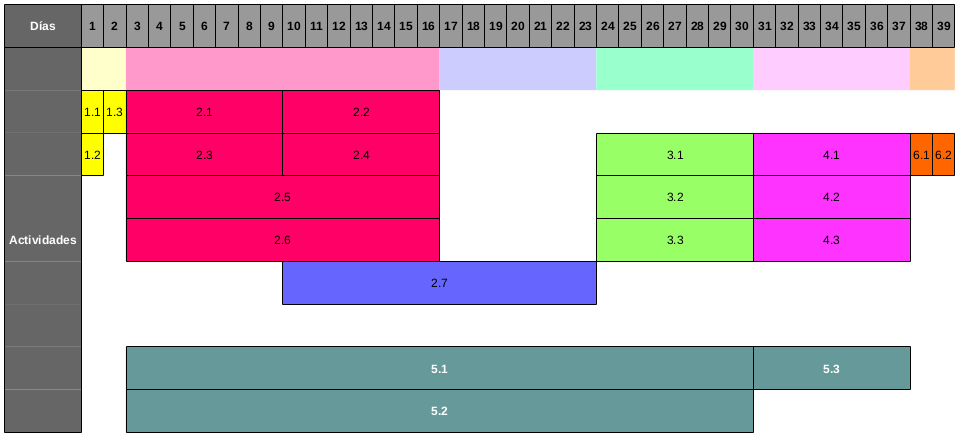
\includegraphics[width=1\textwidth]{Gantt.png}
  \caption{Diagrama de Gantt}
\end{figure}

%%%
\section{Análisis de Riesgo}

\subsection{Posibles problemas}
\begin{itemize}
\item Pérdida de datos
\item Ausencia de integrantes del equipo
\item Imposibilidad de comunicación por incompatibilidad de horario
\end{itemize}

\subsection{Plan de contención}
Para evitar los potenciales riesgos que se pueden presentar a lo largo del desarrollo del proyecto, se opta por trabajar de manera defensiva y prevenir los sucesos con mas probabilidad de ocurrencia.

\begin{itemize}
\item Toda la documentación y código del proyecto será trabajada sobre un repositorio en Github, en donde se podrá observar y obtener métricas de cómo evoluciona el trabajo. De esta manera, cualquier problema de pérdida de datos, será minimizado por el respaldo permanente de cada una de las versiones (con la posibilidad de rastrear cada cambio).
\item Si por algún motivo un integrante del equipo no puede realizar la labor asignada, el líder del proyecto se hará cargo de dicha labor de manera personal.
\item La comunicación se realizará obligatoriamente vía correo electrónico y presencial de manera opcional.
\end{itemize}

\end{document}
